\chapter{Chapter 3 : Problematic and data}\label{chp:3}

\minitoc

Studies on environmental data befalls a multidisciplinary domain called environmental science that regroups various fields such as : physics, biology, chemistry, geography, ecology (and many more that won't be listed here). That important gathering of subjects induced an large collect of data coming from different source of information. As stated in \cite{Manly2008}, the emergence of environmental statistics comes from the obvious fact that much of what is learned on the environment is based on numerical data. Three broad types of areas of studies that we believe it is important to state in this work : 

\begin{itemize}
    \item \textbf{Baseline studies} aim at documenting the present knowledge and how environmental processes operate. Future changes will be define as any deviation from the standards identified by those studies.
    \item \textbf{Targeted studies} intend to characterize and assess the impact of planned or known changes (accidents, human activities). 
    \item \textbf{Regular monitoring} is designed to detect patterns such as variations, trends or changes in important parameters.  
\end{itemize}
In recent years, we can cite numerous applications that can be designated as environmental statistics and they span on a very large specter of problems \cite{BUNCE_2018,Harvell1999,Hoeoek2013,Zheng2021,Zhao2010,Shi2022,Ozgul2010,Mori2012}. 

%Phyto-pharmacovigilance is part of this type of study. It can be formally defined as a vigilance system that collects and analyzes monitoring data on phytopharmaceuticals (pesticides). The aim is to detect adverse effects associated with the use of these products as quickly as possible in order to protect the health of living organisms and ecosystems. This task falls under the responsibility of several agencies in Europe, including the European Food Safety Agency (EFSA), the European Chemical Agency (ECHA) and the European Environment Agency (EEA). In France, this task falls under the responsibility of the Agence nationale de sécurité sanitaire de l’alimentation, de l’environnement et du travail (Anses) i.e. the French Agency for Food, Environmental and Occupational Health \& Safety. Phytopharmacovigilance is an essential complement to the other tasks of the Agency, as one of its main tasks is to regulate by granting or denying authorizations for pesticide products\footnote{All their decision statements are available online \url{https://www.anses.fr/fr/decisions}.}. 

%Data collected or generated as part of phytopharmacovigilance allow to adjust, if necessary, the conditions of authorization for products currently placed on the market, e.g. by reducing the dosage, adjusting the conditions of use or withdrawing an authorization; to initiate management measures to reduce risk exposure, e.g. to protect people in the vicinity of treated areas; to contribute to the development of pre-market risk assessment methodologies used at the European level, if necessary.  

%The Anses does not collect the data it uses directly to accomplish its missions. It relies on its partner network to obtain data sets of interest. This partner network consists of other agencies (national or European), research laboratories, and associations. The decision to add a new source of information first requires a discussion on the coherence of the use of this source of information to provide an answer to the problem under study. For pharmacovigilance, the following information is of interest : 
%\begin{itemize}
%\item Contamination of the environment - air, water, soil, food and drinking water - by residues including metabolites of pesticides.
%\item Exposure, impregnation and effects on living organisms and ecosystems as a whole: humans, livestock and wildlife, crops, flora, etc. Resistance phenomena in organisms targeted by these molecules: Pathogens, weeds, insects.
%\end{itemize}

The purpose of this work is to assist agency experts in their task of monitoring pesticides use and effects on the territory. More precisely our problematic is the following : \textbf{How to locate in time and in space interesting signals from the data at disposal ?} It is essential to make an inventory and a brief description of the data that we will process for their study. To get a general idea of the information that the various data sets can provide, we propose the approach schematized in Figure \ref{fig:compartments}. It is argued that if one knew and controlled all the numerical data in these three compartments and their relationship to each other, one could fully describe the lifetime of a chemical in its application. We divide this diagram into three compartments: 
\begin{itemize}
    \item the emitting source, which corresponds to the knowledge of the dose and the application methods of the considered substance This compartment corresponds to the description of the input data of a diffusion system in a medium.
    \item the diffusion of the substance, which depends on the ambient environment considered. combines information about the structure of the observed environment and the chemical properties of the substance. This compartment describes how the substance moves in a particular environmental medium.
    \item the impregnation and potential undesirable effects, which are simply the exposure and consequences of the substance's introduction into the environment.
\end{itemize}
In practice, we don't have a full control and knowledge of such information. We will see how to get partial information over this circuit in Figure \ref{fig:compartments}. A general overview of the available information will be carried out in Section 1 The description of these data will allow us to identify the specific features and challenges that we will present in Section 2. 

\begin{figure}[ht]
    \centering
    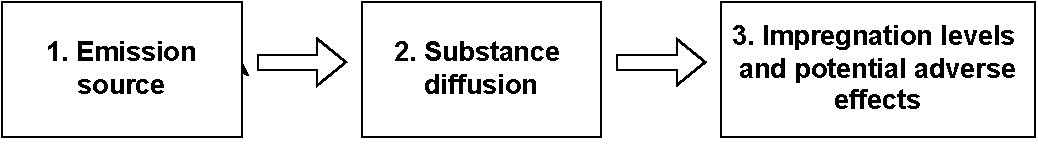
\includegraphics{Chap3/schema1.pdf}
    \caption{Three main compartments of a complete monitoring procedure.}
    \label{fig:compartments}
\end{figure}

\section{General overview}

This section illustrates the variety and scope of data sets that can be used for phytopharmacovigilance. We will show which sources of information we can assign to each of the subjects described in Figure \ref{fig:compartments}. The inventory focuses on all data sets that can provide spatio-temporal information on the evolution of the substance during its emission, its dispersion, and the study of variations in potential adverse effects. We will illustrate several specific cases such as water, air, or soil quality monitoring. We will see that each context requires a selection of information that seems coherent and necessary. Wherever possible, graphical representations of examples will be shown. It is possible that some sources of information necessary for the analysis of certain phenomena are not available as open source. However, the producers of the data in question are systematically cited.

\subsection{Emission source}

The most accurate information about the sources of a substance's emissions could be obtained by quantified, parcel-based tracking of substance consumption. One could imagine a plot with one or more spatial points for each parcel. Each of these points could be linked to a temporal monitoring curve of the tonnage of a substance consumed in the part of the parcel it is located. Such a representation is not possible for several reasons. It is not legally possible to set up a monitoring system with sufficient resolution to identify a parcel owner. The anonymity of those involved in agriculture must be preserved in these investigations. In addition, such a system would only be feasible with considerable sampling effort. Nevertheless, three data sets can provide partial information on the source of pesticide emissions. 

%Specific pest species can be observed for each crop type. Mapping the crop types in an area can therefore provide a preliminary idea of the areas and periods of application of the substance being monitored. Some of this information is available in the graphical land register (GLR) \footnote{Available at : \url{https://www.data.gouv.fr/fr/datasets/registre-parcellaire-graphique-rpg-contours-des-parcelles-et-ilots-culturaux-et-leur-groupe-de-cultures-majoritaire/}.}. This database corresponds to the application forms used by farmers to obtain financial aid under the Common Agricultural Policy of the European Union (CAP). To be eligible for these grants, the crops grown on the plots must be declared. This dataset is a partial information, since the query of CAP is not mandatory. Therefore, the owners of the plots who have not applied for aid are not informed. Moreover, this register is renewed every year. It is possible that the information for certain parcels is not included in all annual editions of the GLR. 

%The use of a substance can also be indirectly seen in the sales data of crop protection products. The National Bank for the Sale of Pesticides by Authorized Distributors \footnote{Available at \url{https://geo.data.gouv.fr/fr/datasets/bdc2c6f21f70acccfea73445f68a5f0d6ee5b7c1}.} (NBSD) lists and archives all such data. For the same reasons of anonymity, geographically fine resolution information is not available. The most accurate resolution corresponds to postal codes. It is the same for the temporal resolution that is not finer than the yearly resolution. Unlike CPL, this data set does not indicate the location and date of use of the substance. A purchaser may well be in a different location than the place of use of the substance they just purchased. Nevertheless, sales give a general indication of the intensity of use of a substance. A sudden increase in sales of a product may mean that its use is increasing in that area.  

%A final source of available information is cultural practice studies. They are conducted in the form of a questionnaire and are used to describe and characterize how farmers work on their land. These studies are very specific and focus only on certain types of crops when conducted. Three topics are addressed in the questionnaires. The first captures general information about the farm, such as commitment to a pesticide use reduction approach or related to agroecology. The second questionnaire is used to reconstruct the technical process on the plot. In other words, we examine the layout of the plot, its preceding crops or its irrigation. Finally, the use of plant protection products on the whole farm is investigated. The type and settings of the sprayer for the substance or the handling and protection of the user are criteria that are interrogated. In summary, cropping practice surveys provide much qualitative (rather than quantitative) information about the source of substance emissions. However, these surveys are conducted on an ad hoc basis and cover only certain types of crops. Only the results of the statistical departments of Agricultural ministry analyses \footnote{An example can be found at :\url{https://agreste.agriculture.gouv.fr/agreste-web/disaron/Chd2009/detail/}.} are available as open source, but not the raw data.  

\subsection{Substance diffusion}

An ideal drug monitoring system would allow the concentration of the monitored molecule to be accurately quantified at any point in its network and at any time. Again, this is not possible in practice, most systems consist of a series of positioned stations at strategic places depending on the environmental medium investigated. Examples of monitoring in three different observing environments are presented here.  

Surface water is water located on top of the Earth's surface, and is defined by opposition to underground waters. It is usually used specifically for terrestrial water bodies and littoral waters, the vast majority of which is produced by precipitation and runoff from nearby higher areas. The propagation of a substance is then assessed by a network of stations positioned on rivers or lakes sides and sampling directly from the water. All records are available on the site of the National Water Data and Repository Administration Service (Sandre\footnote{\url{https://www.sandre.eaufrance.fr/}} and Naïades sites\footnote{\url{https://naiades.eaufrance.fr/donnees-disponibles}}). A coherent geographical source of information to cross with the samples information is the hydrographic network of the area of study. This information is provided by the National Geographical Institute (IGN) \footnote{See :\url{https://geoservices.ign.fr/documentation/donnees/vecteur/bdtopo}}. This network allows to identify which stations are linked by a path of water and the flow direction identify an order between stations (which one is upstream/downstream). It will then provide a better understanding of the temporal dispersion of a substance in the rivers network. Figure \ref{fig:esu_ex} illustrates all stations of the Centre-Val de Loire region that made at least one sampled between 2007 and 2022 and the hydrographic regional network. Another complementary source of information is the hydro-ecoregions. Although the hydrographic network is the information with the most accurate geographic resolution, some parameters not informed by the IGN may influence the diffusion of a pesticide in water. Examples include climatic conditions and riverbed composition. Hydro-ecoregions (HER) are geographic units in which hydrographic ecosystems share common characteristics. The criteria by which they are delineated combine characteristics of geology, terrain, and climate \cite{wasson:hal-02580774}. The National Institute for Agriculture Food and Environment (INRAE) services provided such information\footnote{The open data HER shapefiles : \url{https://geo.data.gouv.fr/fr/datasets/1135b7fd3ca5de69a080f04c31cdc1216a9a34e0}}. The boundaries of these areas are shown in black in Figure \ref{fig:esu_ex}. 

\begin{figure}[ht]
    \centering
    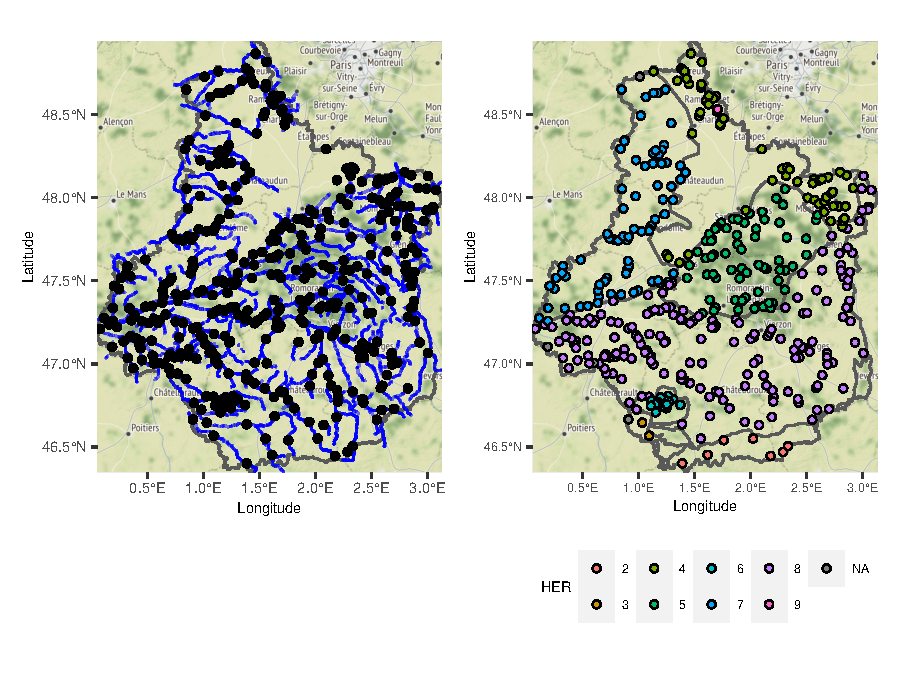
\includegraphics{Chap3/ESU_EX.pdf}
    \caption{Stations monitoring water suface in the Centre-Val de Loire french region. Two different geographical scales are represented. The underlying hydrographic network linking all stations is plotted on the left, the stations are colored according to their hydroecoregion on the right.}
    \label{fig:esu_ex}
\end{figure}

A second example is air quality monitoring. Information on active substance concentrations is collected and available as open source on the website ATMO website\footnote{\url{https://www.atmo-france.org/}}. This website aggregates all data from the regional air quality monitoring agencies (ASQAAs). This example illustrates the fact that the monitoring mission is highly dependent on the monitored environment. This change in propagation medium means that the coherent data sets are no longer the same (it seems fairly obvious that river information does not provide air quality information). Meteorological data is a relevant dataset for this application, especially any information that can be found about wind (wind direction, wind strength, etc.). Historical weather records are now available as open source on the Météo France website\footnote{\url{https://public.opendatasoft.com/explore/dataset/donnees-synop-essentielles-omm/table/?flg=fr&sort=date}}. Figure \ref{fig:air_ex} illustrates the cross-referencing of data from air quality monitoring stations with meteorological data.

\begin{figure}[ht]
    \centering
    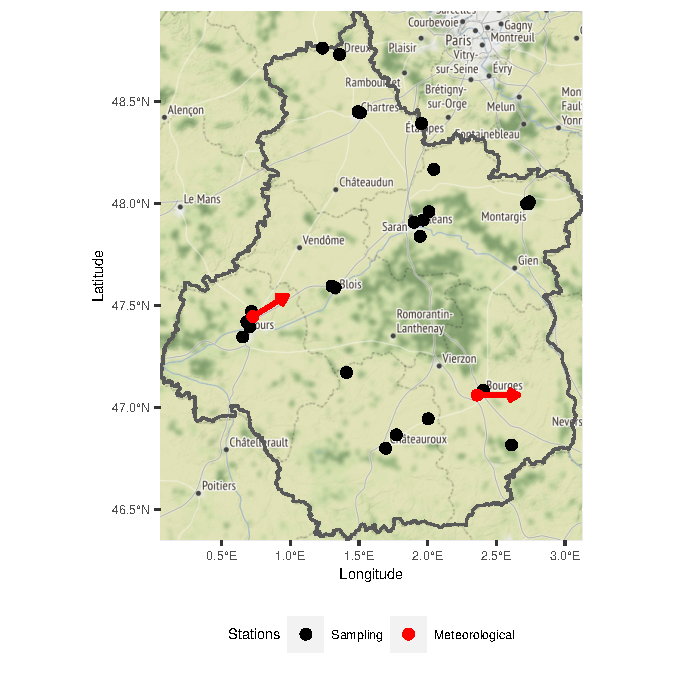
\includegraphics{Chap3/AIR_EX_DATA.pdf}
    \caption{All active stations measuring air quality on March the 1st of 2021 coupled with meteorological stations active that day. The main wind direction and speed measured that day is mapped with the red arrows.}
    \label{fig:air_ex}
\end{figure}

The last example shows that environmental compartments are very different. The agency may also be interested in the quality of water for human use. Unlike the previous examples, the selection of consistent data sets for the study of this environmental medium is less obvious. Three main functions can be distinguished in a drinking water system \cite{renaud:hal-01218670}. The first corresponds to the sampling and collects all information about the raw water resource. The second one defines the production of the drinking water, i.e. its transport, storage and eventual treatment. The distribution to the user is the last function. In order to obtain information that allows the observation of these three functions, the required data sets must be diverse and of different nature.  The sampling part is observed using information on the quality of the raw water and therefore requires data sets on environmental quality (as in the previous two examples). The other two functions, on the other hand, are related to human activities and therefore require a completely different spatial approach. For example, observation at the administrative level (e.g., departmental level) is consistent. If finer resolution is desired, we can consider water management units (WMUs) or other scales described in \cite{renaud:hal-01218670}. All the data is provided by the Department of Health\footnote{Open source data at: \url{https://www.data.gouv.fr/fr/datasets/resultats-du-controle-sanitaire-de-leau-du-robinet/}.}. 

Thus, it is clear that each environmental compartment is examined using a variety of data sets. The list in this section is not exhaustive. We can add to it the study of soil quality, food production and distribution, animal feed, groundwater, indoor air and dust... In particular, we note that the spatial analysis of the dispersion of a substance in an environment depends very much on the observed network and the mechanisms that govern that environment. For example, the hydrographic network of a region depends both on the natural geography of the area and on human activity (presence of irrigation canals in the network), while the distribution units of water intended for human consumption are entirely determined by human activity. 
 
\subsection{Impregnation levels and potential adverse effects}

Once a pesticide has been applied and has spread in an environmental compartment, it is interesting to observe how ecosystems are affected by the active substance. Two aspects can be distinguished: the exposure to which ecosystems are subjected, i.e., their impregnation, and the possible adverse effects that result. As is often the case in statistics \cite{shipley2016}, it is complicated to identify direct relationships between cause and effect. Rather, these two aspects are linked through correlational relationships. The data sets are not of the same type. Several examples of datasets illustrating those two aspects are given here. Very few data are available as open source, as they all fall under the General Data Protection Regulation (GDPR). We therefore limit ourselves to mentioning the names of the actors responsible for the collection of the data and to giving a general overview of the content of the data.

Concerning the impregnation of the environment, the main issue here is measuring the concentration of active ingredients in the living organisms that make up the exposed ecosystems. For example, the Anses, in collaboration with Santé Publique France, will be conducting a new study called Pestiriv \footnote{see full description here :\url{https://www.anses.fr/fr/content/lancement-de-pestiriv-une-\%C3\%A9tude-in\%C3\%A9dite-sur-l\%E2\%80\%99exposition-aux-pesticides-des-personnes-vivant}} on this topic in the coming months. In France, a large part of the rural population lives in wine-growing areas, which explains the importance of this project. As part of this study, hair and urine samples will be taken from people living in wine-growing areas. This will allow the exposure of farmers to pesticides to be measured. The deposition of pesticides in bee matrices is another example of impregnation. The Technical and Scientific Institute of Apiculture and Pollination (ITSAP) is the institute responsible for monitoring this environmental medium. We look for pesticide concentrations in pollen in beehives..

The databases for monitoring potential adverse events are medical registries. There are human and animal health databases. For human health, the Phytattitude network was developed by the Mutual Agricultural Health Insurers (MSAs). It is a network where any professional who comes into contact with phytosanitary products can indicate if he/she has health problems. This organization collects data through spontaneous reports from agricultural actors or during scheduled visits by nurses or doctors. Another source is the medical-administrative databases of the MSA. They collect information on farmers' health care reimbursements. Second, poison control centers are involved in adverse effect surveillance. They provide toxicovigilance information on toxicovigilance for the entire population. Much information about acute health problems comes up through these information channels. For chronic health problems, there is the National network of vigilance and prevention of professional pathologies (RNV3P), whose role is to identify emerging or re-emerging occupational health risks. Finally, the AGRICAN cohort (AGRIculture and CANcer) of the François Baclesse Center is used to measure the health status of the agricultural population compared to the general population (especially in terms of cancer burden). It is therefore also part of the Anses partner network of partners. Regarding animal health, INRAE provides a database on veterinary toxicovigilance (GIS Toxinelle), and the Biodiversity French Office (OFB) on wildlife toxicovigilance of wildlife. The Department of Agriculture provides additional information, such as acute mortality in bees, and its 500 ENI biovigilance program is also part of the available databases. This is a program to monitor the impact of agricultural practices on biodiversity.

This section explains the diversity of the actors that are involved in a partnership with the Anses and the extent of the number of data sets that can be of use in a monitoring mission. It also highlights the need for regular discussion with experts to identify and properly manipulate this information. In this work, we made a selection of datasets focused on surface water monitoring. This allowed us to narrow down the many possible research directions and frame the work done in this thesis. Figure \ref{fig:compartments_choice} summarizes the datasets that were selected to develop an algorithm for detecting anomalous spatiotemporal signals in surface waters. This scheme is presented in section 5. Impregnation and adverse effects data are not available, so this aspect of the monitoring scheme is not addressed.

\begin{figure}[ht]
    \centering
    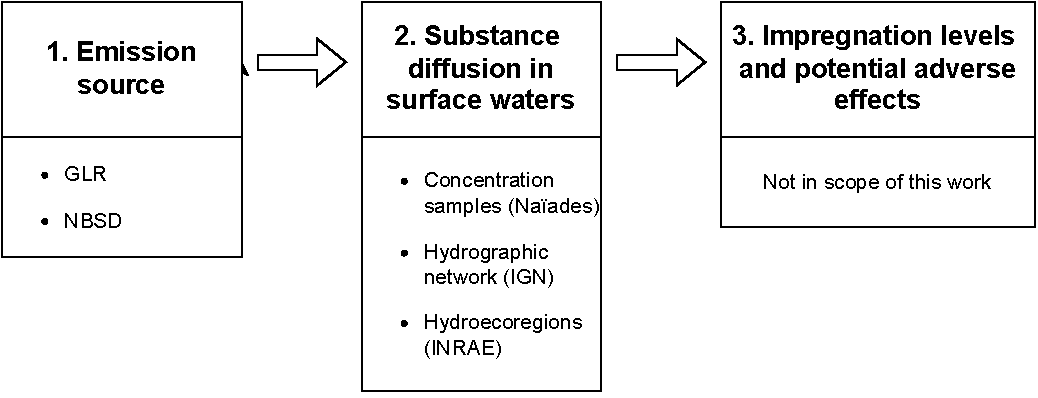
\includegraphics{Chap3/schema2.pdf}
    \caption{Data sets selected in this work.}
    \label{fig:compartments_choice}
\end{figure}


\section{Environmental data specificity}

Although the sources of information used to develop models vary, common features can be identified. Three aspects of different nature are presented in this section. All illustrations are made with data of prosulfocarbe concentration in the Centre-Val de Loire french region. 

\subsection{Inherent data characteristics}

%The first specificity of concentration measurement arises from the problem of measuring a chemical substance in a sample. In applied chemistry, any measuring device is characterized by two types of limits. 

%\begin{itemize}
%    \item The detection limit (LOD): This is the smallest concentration value in a sample that can be distinguished from zero with certainty.
%    \item The limit of quantification (LOQ): This is the smallest concentration value of a substance in a sample that can be measured with certainty. 
%\end{itemize}

%It is important to know that these two limits are determined by the instrument that performs the measurement. It happens that geographical areas are covered by stations that do not have the same equipment. In this case, there are several LOQ values within the samples taken in that area. In the case of surface waters, for example, the contracts for the selection of monitoring laboratories are awarded by the water agencies. These agencies, six in number, cover an area larger than the French administrative regions. This means that if the scale of an administrative region is taken as the basis for a study, this region may fall under the jurisdiction of two different water agencies and therefore the measuring instruments may be different. Moreover, the same station may change its measuring equipment over time. Station equipment contracts are renewed periodically, but renewal does not guarantee that the same equipment will be maintained. All those caracteristics are illustrated in Figure \ref{fig:cens_ex}. These two limits of accuracy mean that concentration data are left-censored. However, unlike the classical censoring problems described in the literature, the values of the censoring thresholds are known. Several methods have been developed to handle this type of data. We can cite the imputation of values to replace the LOQ values present in the set of concentration values, the use of the maximum likelihood estimator or the Kaplan-Meier estimator (see \cite{Gillaizeau2020,Croghan2003MethodsOD}). In Chapter 4, we will show which method was chosen to handle this type of data in this thesis. 

%\begin{figure}
%    \centering
%    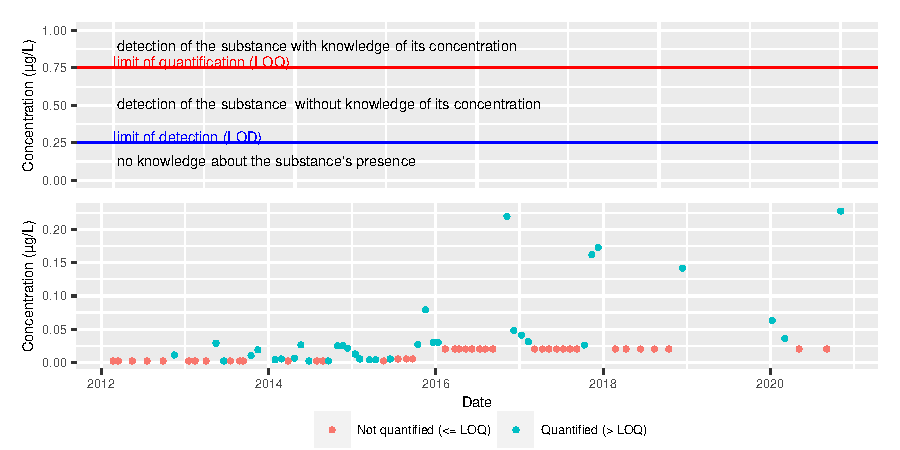
\includegraphics{Chap3/Cens_ex.pdf}
%    \caption{Censorship illustration. The top Figure sums up the limits of measurements effects. The bottom Figure shows the consequences of censorship on the samples of a station located in the Centre-Val de Loire region. This station changed its equipment in 2016, the LOQ change values.}
%    \label{fig:cens_ex}
%\end{figure}

The concentration data also show strong tails in their distribution. In Figure \ref{fig:shape_ex} there are not only many low concentration values (corresponding to the measured values that did not exceed the quantification threshold), but also high concentration values. The maximum value is almost 3 µg/L. The data used in Figure \ref{fig:shape_ex} are the measured values from a period when the substance in question was typically used. This ensures that we have a high quantification rate and thus many fully observed samples. The concentration data can therefore be summarized as left-censored heavy-tailed data.

\begin{figure}[ht]
    \centering
    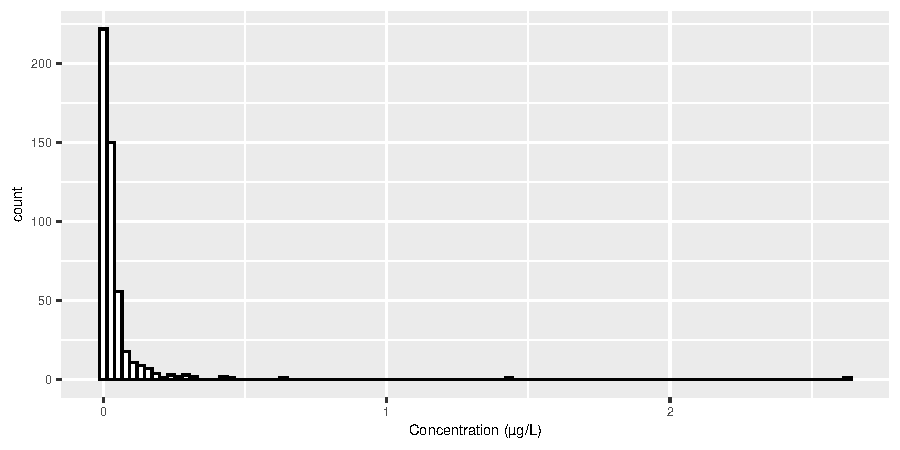
\includegraphics{Chap3/Shape_ex.pdf}
    \caption{Histogram of all measurements of prosulfocarbe made between 2017-10-01 and 2018-02-01 in the Centre-Val de Loire region.}
    \label{fig:shape_ex}
\end{figure}

\subsection{Heterogeneity in distribution and sampling rates}

%The second feature of these data is the spatial and temporal heterogeneity of the measurements. This is not the case for all pesticide monitoring data. This makes it a particularity of the French network. Figure \ref{fig:cens_ex} already shows that the rhythm of the measurements for the same station is irregular in time. Figure \ref{fig:het_samp_ex} shows that for two spatially neighbouring stations the measured values are not synchronous in time. It can also be seen that the stations take very few measurements and do not take the same number of measurements. In Figure \ref{fig:het_samp_ex} we see that it is not possible to compare the measurements of the two existing stations. The stations literally sampled in non-overlapping time periods. Therefore, to derive information from these data, one must work on a different scale than that of the station. Aggregating the data from the two stations results in a time series that is more evenly sampled over time. Thus, there is a trade-off between the number of data available to make a statistical statement about a spatial area and the accuracy of that spatial extent. 

%\begin{figure}[ht]
%    \centering
%    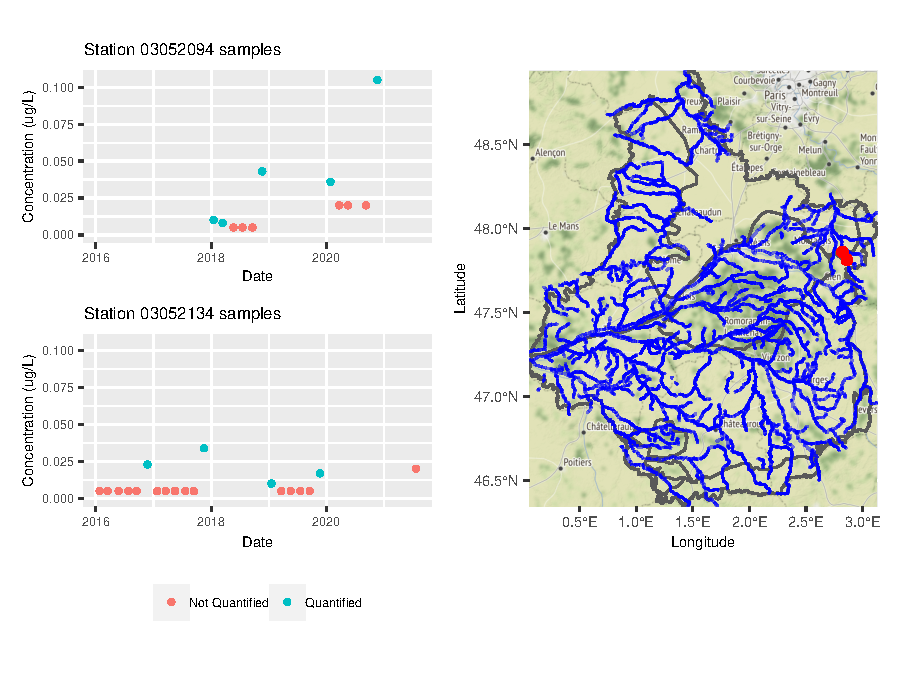
\includegraphics{Chap3/Hetero_ex.pdf}
%    \caption{Spatial and temporal heterogeneity in sampling. The Figures on the left represent all the samples of two neighbouring stations. The map on the right shows the position of those stations.}
%    \label{fig:het_samp_ex}
%\end{figure}

%Figure \ref{fig:het_spa_ex} illustrates that alongside heterogeneity in the stations sampling rhythms, spatio temporal data are not distributed in a homogeneous way over the territory. Depending on which region of the area of study the samples originate, the underlying distribution differ. Thus, the data are heterogeneous in space. This Figure also illustrates that the distribution of concentration values can drastically change over time. Looking at the samples of station 03189000, there is a break point just before the year 2015 in the station concentration values. The same can be saif for the year 2016 in Figure \ref{fig:cens_ex}. Thus the data are heterogeneous in time. The spatio-temporal heterogeneity affects the sampling rhythms and the distribution of the concentrations. 

%\begin{figure}[ht]
%    \centering
%    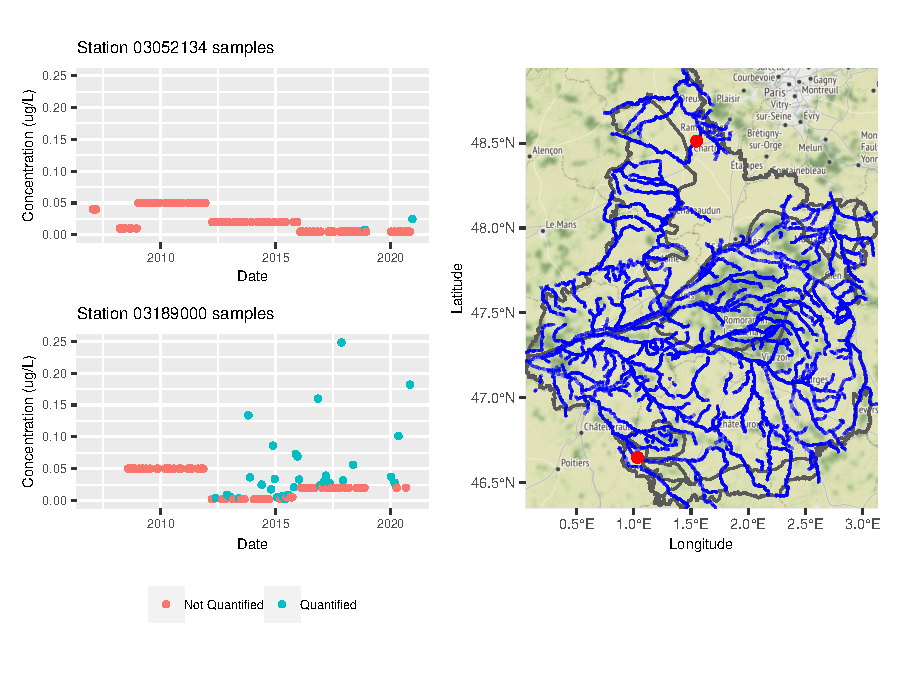
\includegraphics{Chap3/het_spa_ex.pdf}
%    \caption{Spatial and temporal heterogeneity in distribution. The Figures on the left represent all the samples of two stations. The map on the right shows the position of those stations.}
%    \label{fig:het_spa_ex}
%\end{figure}

\subsection{Representation}

%The final problem associated with spatiotemporal data is their representation. The minimum number of dimensions to describe them is three: two for space as a pair of longitudes and latitudes; one for time. \cite{cressie2015} presents in his book several methods of descriptive statistics for the representation of such data. The most intuitive method to plot spatiotemporal data are marginal and conditional plot. There are several ways to make them.

% The first one are \textbf{time-series plot}. The figures presented so far in this section are one possible example of this representation where one commits to a geographic position for observing a time series. Figure \ref{fig:tsplot_ex} displays the daily maximal concentrations of prosulfocarbe in three adjacent hydroecoregions (report to Figure \ref{fig:esu_ex} for spatial representations of the HER). Clear correlation is observed between the time series. However, the signal of HER 4 doesn't seem to be exactly the same and shows earlier signs of a seasonal pattern and of higher quantified values. Another example is shown in Figures \ref{fig:het_spa_ex} and \ref{fig:het_samp_ex} that allowed to see the spatial heterogeneity of sampling rates and distribution. The problem is that we cannot get a complete view of the spatial distribution of the data. The stations compared in both figures were hand-selected, and no information is available about the others. By selecting the HER scale, we insert expert information in the visualisation. Note that each choice has its advantages and its drawbacks. For instance, if looking at HER 4 in Figure \ref{fig:esu_ex}, stations that belong to it are separated in three clear clusters (one in the north, the other in the east and last one in the south west of the HER). As though they belong to the same HER, grouping the data of these stations is not necessarily an ideal choice as they are still far away.. 
 
% \begin{figure}[ht]
%    \centering
%    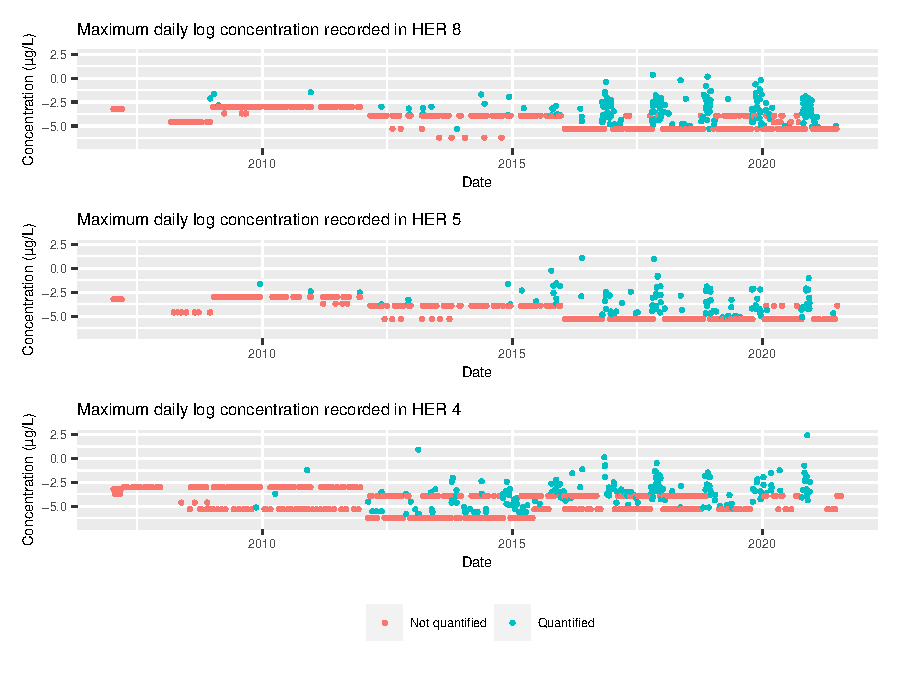
\includegraphics{Chap3/TS_plot.pdf}
%    \caption{Time series plot of HER 8,5 and 4 daily maximum concentrations. The log scale was used for a easier visualization.}
%    \label{fig:tsplot_ex}
%\end{figure}
 
% Second, the \textbf{spatial maps plot} can also be an effective way of extracting information from these data. It consists in a temporal sequence of maps as in Figure \ref{fig:spa_ex}. A clear seasonal pattern can be identified from this Figure. Two problems emerge from this representation method. First, it takes an extensive number of maps to exhibit significant patterns. Secondly, the four seasons of the year were chosen to make a temporal segmentation of the two observations year. We introduced external knowledge to our analysis, Same as previously, even though it is a coherent choice, it has it s drawbacks. For instance, it cannot take into account the years where treatment started earlier or later due to climatic conditions. Furthermore, it can't help to determine precisely the nature of what is temporally changing in the signal. only the summarised indicator of quantification rate is used. Nothing is known about the maximum or the mean concentrations. Plotting all the maps displaying other indicators would be a tedious task.   

%\begin{figure}[ht]
%    \centering
%    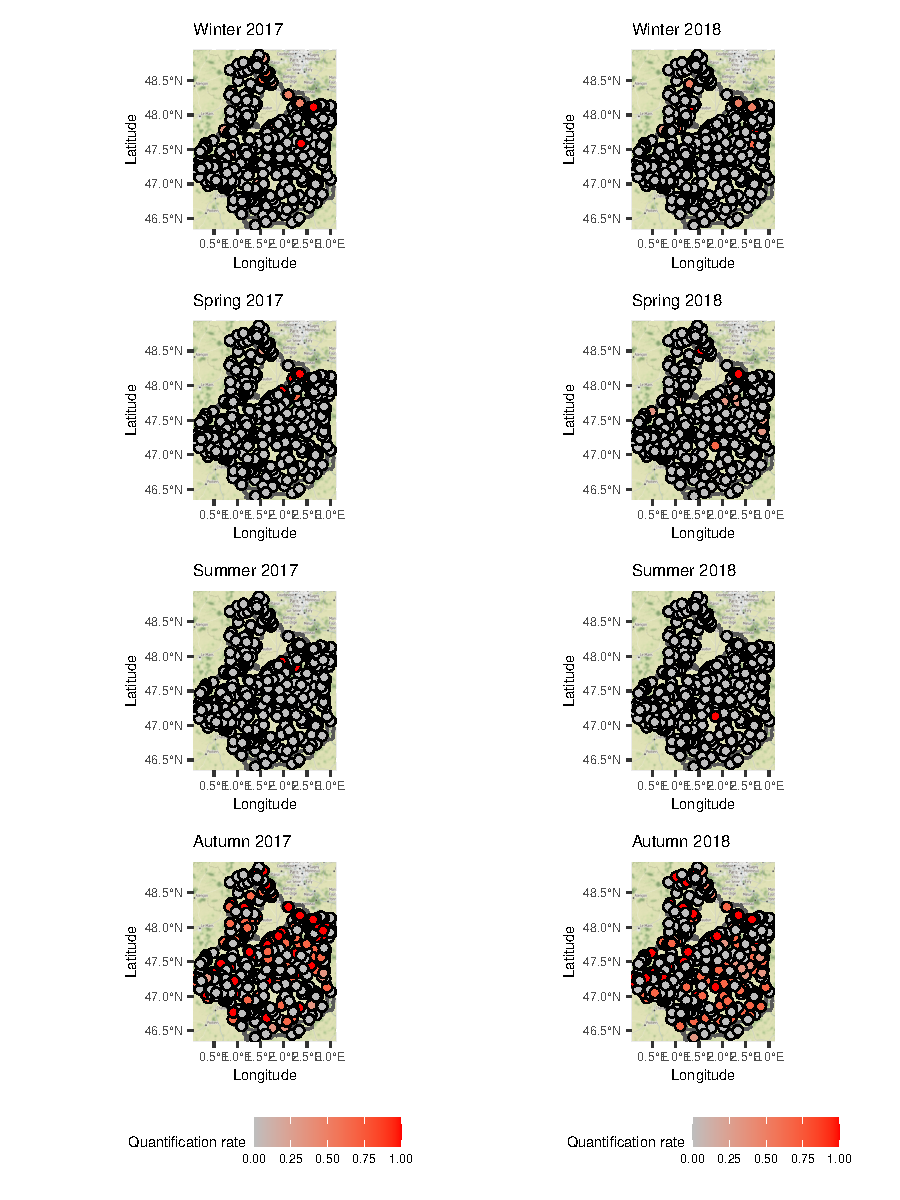
\includegraphics{Chap3/Spatial_maps.pdf}
%    \caption{Spatial maps in time. The prosulfocarbe's quantification rate of each station was computed for each season of 2017 and 2018.}
%    \label{fig:spa_ex}
%\end{figure}

%Another example of representation is the \textbf{space (1-D)/time plots} shown in Figure \ref{fig:S1Dplot}. It consists in fixing a dimension in space whether longitude or latitude and to plot some indicators summarised on that dimension against time. In Figure \ref{fig:S1Dplot}, the longitude was cut into regular intervals and time was segmented in seasons. The plot shows once again a very clear temporal seasons that appears in time in the region. The location of those changes are not clearly displayed by those plots though. We are not able to determine if the large quantification rates are in the central areas of the region or not (given that we miss the latitude information). Although those plots provide an excellent first overview and can help to quickly understand the structure under spatiotemporal data, it does not provide sufficient precision to localize in space and time some interesting signals.    

%\begin{figure}[ht]
%    \centering
%    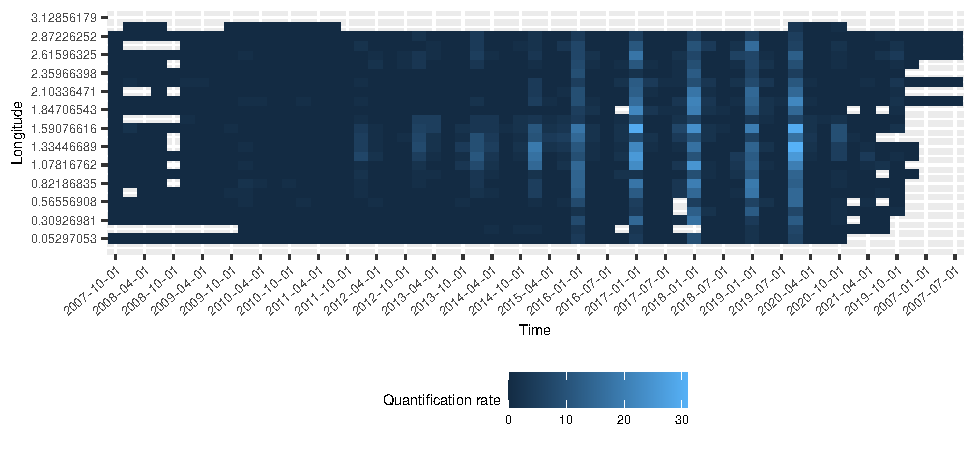
\includegraphics{Chap3/T1Dplot.pdf}
%    \caption{Space (1-D)/Time plots. Grey tiles correspond to location and moment were no sample were collected.}
%    \label{fig:S1Dplot}
%\end{figure}

%All of those representation methods can't capture all the information carried by the data set. We propose to handle it in a dynamic way using the application environment R-shiny. Integrating dynamic response to a user's requests is an efficient way to combine a descriptive view with models results. The application overview will be given in section 6.
